\section{Marco teórico, conceptos clave del ML}

\begin{quote}
    `\gls{ml}: the use and development of computer systems that are able to learn and adapt without following explicit instructions, by using algorithms and statistical models to analyse and draw inferences from patterns in data'\ \cite{machinel18:online}
\end{quote}

Es decir, un sistema que es capaz de inferir patrones de unos datos y realizar predicciones sobre nuevos datos a raíz de los patrones encontrados. 


\subsection{Tipos de aprendizaje y modelos}

Hay cuatro tipos de aprendizaje en el ML:\@ supervisado, no supervisado, semi-supervisado y de refuerzo\ \cite{homl56}.

Como parte de nuestros datos están etiquetados, podemos utilizar tanto el aprendizaje supervisado como el semi-supervisado. En un sistema supervisado se requiere que todos los datos estén etiquetados con la categoría deseada, en nuestro caso la contaminación. Sin embargo, para el semi-supervisado no es necesario que todos los datos estén etiquetados, pues utilizan tanto los datos etiquetados como los que no (datos parcialmente etiquetados) para tratar de generalizar mejor\ \cite{homl56}.

No utilizaremos el no supervisado, pues consiste en un conjunto de técnicas utilizadas para agrupar automáticamente datos no etiquetados a base de similitudes sin tener supervisión previa. El objetivo es que los datos dentro de un mismo grupo sean más similares entre sí que con los otros grupos\ \cite{Clustera13:online}. Sin embargo, como tenemos una cantidad más o menos considerable de información etiquetada, no nos hace falta.

Tampoco utilizaremos el aprendizaje por refuerzo, pues no se encuentra implementado dentro de la librería que utilizamos \textit{\href{https://scikit-learn.org/stable/}{sklearn}} y tampoco está dentro de los objetivos del proyecto.


\subsection{Fases del desarrollo de un proyecto de ML}

Nuestro proyecto ha tenido las fases que nombramos a continuación:

\begin{enumerate}
    \item Obtención de datos (\textit{apartado\ \ref{sec:obtencion}})
        \begin{enumerate}
            \item Recolección de información de los \acrshort{bil}.
        \end{enumerate}
    \item Preparación de datos (\textit{apartado\ \ref{sec:preprocesado}})
        \begin{enumerate}
            \item Selección de métodos de preprocesado
        \end{enumerate}
    \item Entrenamiento de los modelos (\textit{apartado\ \ref{sec:entrenamiento}})
        \begin{enumerate}
            \item Entrenamiento `básico' de modelos
            \item Selección y refinamiento
        \end{enumerate}
    \item Evaluación de resultados
        
    \item Monitoreo de los modelos
\end{enumerate}

Podemos generalizar los procesos de un proyecto de \gls{ml} meidnate el esquema de la \textit{Figura\ \ref{fig:ml-development-cycle}}. Cabe destacar que el proceso de entrenar un modelo de \gls{ml}, como bien muestra la imagen, es un proceso cíclico en búsqueda de mejores resultados a base de probar metodologías distintas, añadir pasos, el cambio de requisitos, etc.

\begin{figure}[!htb]
    \centering
    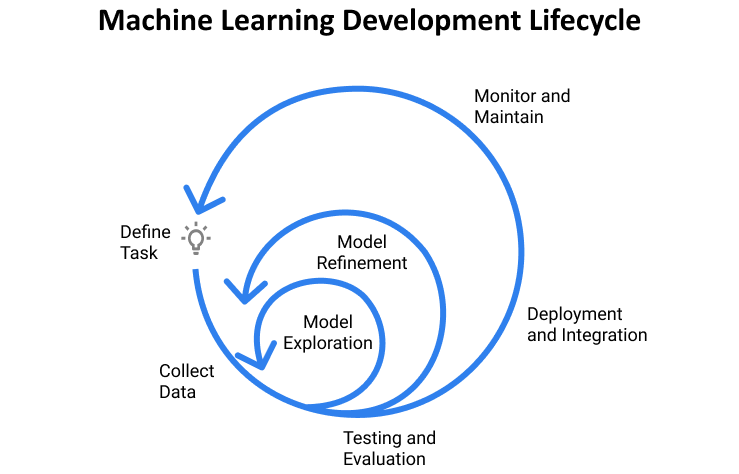
\includegraphics[width=\linewidth]{media/images/ml-development-cycle.png}
    \caption{Esquema del proceso del desarrollo de un proyecto de \gls{ml}, fuente\ \cite{Organizi22:online}}\ \label{fig:ml-development-cycle}
\end{figure}


\subsection{Métricas de evaluación de modelos}

Antes de continuar con el entrenamiento de modelos, su mejora y la selección de pasos del preprocesado; necesitamos algún tipo de métrica para evaluar y comparar los resultados. A continuación, explicaremos las que hemos utilizado para los diferentes tipos de modelos.

\subsubsection{Clasificación supervisada y semi-supervisada}\ \label{sec:classification-metrics}

Primeramente, explicaremos las partes de una matriz de confusión como la que podemos ver en la \textit{Figura\ \ref{fig:confusion-matrix-example}}. Podemos ver que tiene cuatro partes:

\begin{itemize}
    \item \textit{True Positive (tp)}, las muestras que el modelo clasifica como positivas que realmente son positivas.
    \item \textit{False Positive (fp)}, las muestras que el modelo clasifica como positivas que realmente son negativas.
    \item \textit{True Negative (tn)}, las muestras que el modelo clasifica como negativas que realmente son negativas.
    \item \textit{False Negative (fn)}, las muestras que el modelo clasifica como negativas que realmente son positivas.
\end{itemize}

Estos cuatro valores son la base del resto de métricas que comentaremos a continuación.

\begin{figure}[!ht]
    \centering
    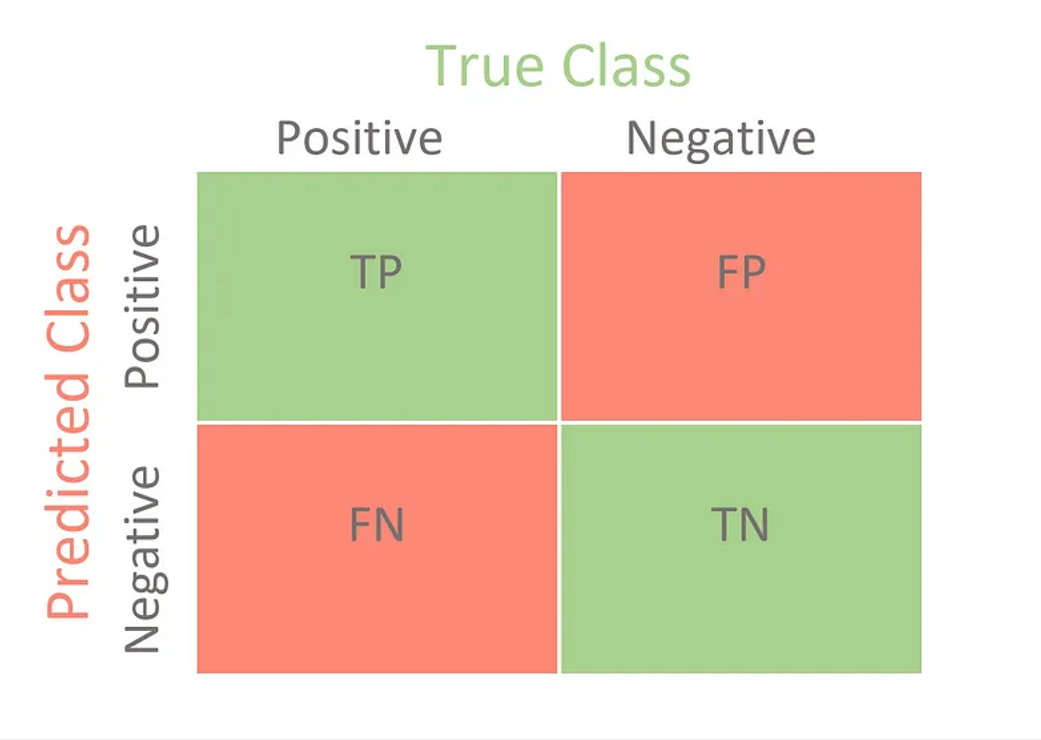
\includegraphics[width=0.7\linewidth]{media/images/confusion-matrix-example.png}
    \caption{Ejemplo de matriz de confusión, fuente\ \cite{Confusio71:online}}\ \label{fig:confusion-matrix-example}
\end{figure}

Antes de continuar con las métricas que compararemos, comentaremos también otras más básicas que son utilizadas para calcular las que utilizaremos\ \cite{Precisio23:online}.
\\ \textit{\textbf{Sensitivity}} permite saber la probabilidad de que una predicción positiva sea realmente positiva.
    \begin{equation}
        sensitivity=tp/(tp+fn)
    \end{equation}
\textit{\textbf{Specificity}} permite saber la probabilidad de que una predicción negativa sea realmente negativa.
\begin{equation}
        specificity=tn/(tn+fp)
    \end{equation}
\textit{\textbf{Recall}} indica la capacidad del modelo para encontrar todas las muestras positivas. 
    \begin{equation}
        recall=tp/(tp+fn)
    \end{equation}
\textit{\textbf{Precision}} indica la precisión de las predicciones positivas, es decir, la habilidad del clasificador para no predecir como positiva una muestra que es negativa.
    \begin{equation}
        precision=tp/(tp+fp)
    \end{equation}

Con estas métricas básicas podemos definir las que realmente compararemos, ya que tienen en cuenta el balanceo del \gls{dataset}:

\textit{\textbf{fbeta score}} es la media harmónica ponderada entre \textit{\textbf{Precision}} y \textit{Recall}. 
El parámetro \textit{beta} representa la importancia de \textit{Recall} por encima de \textit{Precision}. 
Es decir, \(beta>1\) le da más importancia a \textit{Recall} y, contrariamente, \(beta<1\) le da más peso a \textit{Precision}.\ \cite{FscoreWi30:online}
    \begin{equation}
        f_\beta = (1 + \beta^2)*\frac{precision*recall}{(\beta^2*precision)+recall}
    \end{equation}

Para comparar los modelos utilizaremos el parámetro \textit{beta} con valor de \textit{2}, pues consideramos más importante el \textit{Recall}, ya que creemos que los falsos negativos son peores que los falsos positivos. Es decir, consideramos peor que el modelo no detecte una muestra contaminada que detecte una muestra como contaminada cuando no lo es.

\textit{\textbf{Balanced accuracy}} es la media aritmética de \textit{Sensitivity} y \textit{Specificity}. Se utiliza principalmente cuando tratamos con datos desbalanceados.\ \cite{Balanced44:online} Su valor representa la exactitud media del modelo en las diferentes clases representadas por los datos, en nuestro caso, la clase de ``CONTAMINADO'' o ``NO CONTAMINADO''. Este valor, representa la exactitud con la que el modelo es capaz de clasificar las muestras de las diferentes clases, teniendo en cuenta la distribución de la clase mayoritaria. Es decir, si el valor de \textit{balanced accuracy} se acerca al 1, el modelo es capaz de clasificar correctamente las muestras de las diferentes clases, mientras que si se acerca a 0, el modelo no es capaz de clasificar correctamente las muestras o se aprovecha del desbalance de los datos, prediciendo mucho más la clase mayoritaria.
\begin{equation}
    balanced\_accuracy =\frac{sensitivity + specificity}{2}
\end{equation}
